\section{Background and Preliminaries}
\label{sec:bg}

This section introduces our running example, necessary background of ML system internals, as well as common types of redundancy.

\subsection{Running Example}

Example~\ref{ex:1} shows a user-level example ML pipeline---written in SystemDS' DML scripting language with R-like syntax \cite{BoehmADGIKLPR20}---which we use as a running example throughout this paper.

\begin{example} [GridSearch LM] \label{ex:1} We read a feature matrix \mat{X} and labels \mat{y}, and extract 10 random subsets of 15 features. For each feature set, we tune the linear regression (lm) hyper-parameters regularization, intercept, and tolerance via grid search and print the loss.
\begin{lstlisting}
 1: X = read('data/X.csv'); # 1M x 100
 2: y = read('data/y.csv'); # 1M x 1
 3: for( i in 1:10) {
 4:   s = sample(15, ncol(X));
 5:   [loss, B] = gridSearch('lm', 'l2norm',
        list(X[,s],y), list('reg','icpt','tol'),...);
 6:   print("Feature set ["+toString(s)+"]: "+loss);
 7: }
\end{lstlisting}
High-level primitives like \texttt{gridSearch} and \texttt{lm} are themselves script-based built-in functions and imported accordingly. Below functions show their key characteristics in simplified form:
\begin{lstlisting}
01: gridSearch = function(...) return(...) {
02:   HP = ... # materialize hyper-parameter tuples
03:   parfor( i in 1:nrow(HP) ) { # parallel for
04:     largs = ... # setup list hyper-parameters
05:     rB[i,] = t(eval(train, largs));
06:     rL[i,] = eval(score, list(X,y,t(rB[i,])));
07: } }
08: lm = function(...) return(...) { 
09:   if (ncol(X) <= 1024)  # select closed-form
10:     B = lmDS(X, y, icpt, reg, verbose);
11:   else                  # select iterative
12:     B = lmCG(X, y, icpt, reg, tol, maxi, verbose);
13: } 
14: lmDS = function(...) return(...) {
15:   if (icpt > 0) {
16:     X = cbind(X, matrix(1,nrow(X),1));
17:     if (icpt == 2)
18:       X = scaleAndShift(X); # mu=0,sd=1
19:   } ...
20:   A = t(X) %*% X + diag(matrix(reg,ncol(X),1);
21:   b = t(X) %*% y;
22:   beta = solve(A, b);
23: } 
24: lmCG = function(...) return(...) {
25:   if (icpt > 0) {
26:     X = cbind(X, matrix(1,nrow(X),1));
27:     if (icpt == 2)
28:       X = scaleAndShift(X); # mu=0,sd=1
29:   } ...
30:   while (i<maxi & norm_r2>norm_r2_tgt) {
31:     q = t(X) %*% (X %*% ssX_p); ...
32:     p = -r + (norm_r2 / old_norm_r2) * p;
33: } }
\end{lstlisting}
The \texttt{gridSearch} function enumerates and materializes all hyper-parameter combinations $\mat{HP}$ of the passed parameters and value ranges, and invokes training (\texttt{lm}) and scoring (\texttt{l2norm}) functions to find the best model and loss. The \texttt{lm} function in turn dispatches---based on the number of features---either to a closed-form method with $\mathcal{O}(m\cdot n^2 + n^3)$ complexity (\texttt{lmDS}); or an iterative conjugate-gradient method with $\mathcal{O}(m \cdot n)$ per iteration (\texttt{lmCG}), which performs better for many features as it requires $\leq n$ iterations until convergence.
\vspace{-0.1cm}
\end{example}

\subsection{ML Systems Background}
\label{sec:mlsys}

There is a variety of existing ML systems. Relevant for understanding this paper, are especially the underlying techniques for program and DAG compilation, and operator scheduling~\cite{2019Boehm}. Here, we focus primarily on lazy evaluation and program compilation.

\textbf{Program/DAG Compilation:} We distinguish three types of compilation in contemporary ML systems: (1) interpretation or eager execution, (2) lazy expression or DAG compilation, and (3) program compilation. First, interpretation as used in R, PyTorch \cite{PaszkeGMLBCKLGA19}, or Python libraries like NumPy \cite{WaltCV11} or Scikit-learn \cite{PedregosaVGMTGBPWDVPCBPD11} execute operations as-is and the host language (e.g., Python) handles the scoping of variables. Second, systems like TensorFlow \cite{AbadiBCCDDDGIIK16}, OptiML \cite{SujeethLBRCWAOO11}, and Mahout Samsara \cite{MahoutSamsara} performing lazy expression evaluation that lazily collects a DAG of operations, which is optimized and executed on demand. Some of these systems---like TensorFlow or OptiML---additionally provide control flow primitives, integrated in the data flow graph. Here, the host language still interprets the control flow, and thus, unrolls operations into a larger DAG. However, recent work like AutoGraph \cite{abs-1810-08061} automatically compiles TensorFlow control flow primitives. Only bound output variables leave the scope of expression evaluation. Third, program compilation in systems like Julia \cite{BezansonEKS17}, SystemML \cite{BoehmDEEMPRRSST16}, SystemDS~\cite{BoehmADGIKLPR20}, and Cumulon \cite{HuangB013} compiles a script into a hierarchy of program blocks, where every last-level block contains DAGs of operations. Accordingly, control flow and variable scoping is handled by the ML system itself. Despite the large optimization scope of lazy expression evaluation and program compilation, unnecessary redundancy cannot be fully eliminated via code motion and common subexpression elimination (CSE) because the conditional control flow is often unknown.

\begin{figure}[!t]
	\centering
	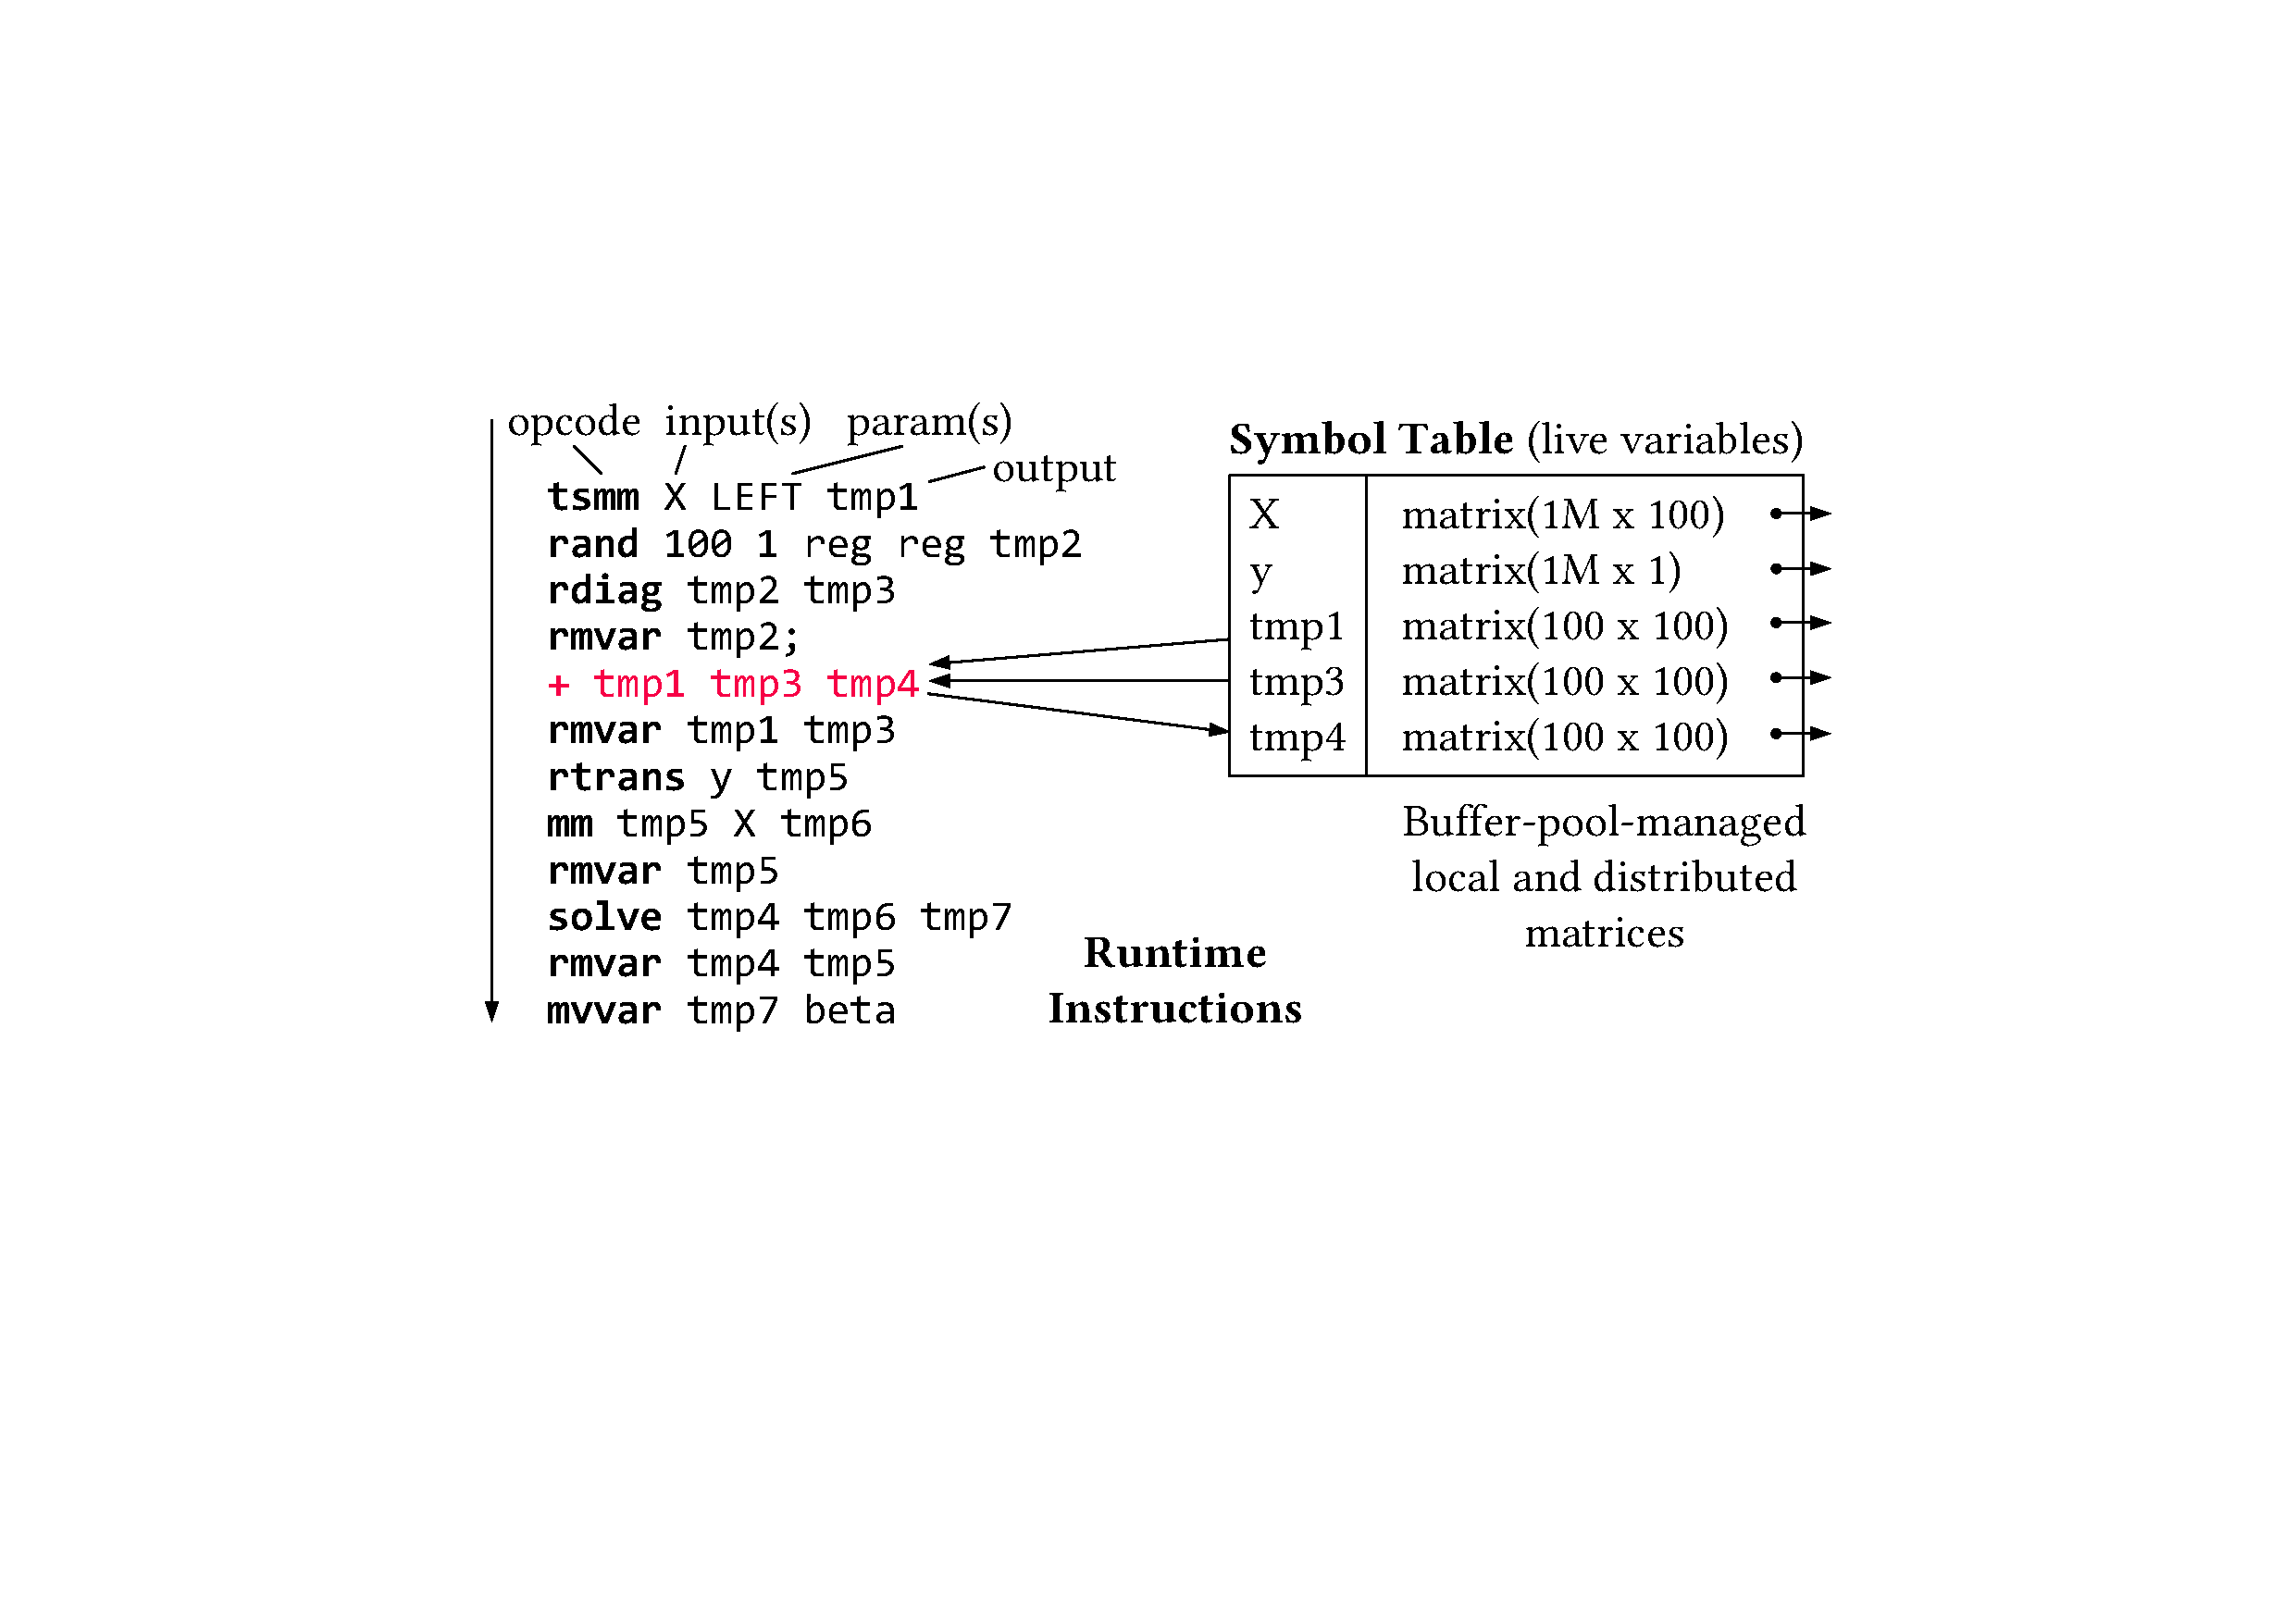
\includegraphics[scale=0.32]{figures/background}
	\vspace{-0.25cm}
	\caption{\label{fig:background}Operator Scheduling and Runtime Plans.}
\end{figure}

\textbf{Operator Scheduling:} Given a DAG of operations of an expression or program block, operator scheduling then determines an execution order of the individual operations, subject to the explicit data dependencies (i.e., edges) of the data flow graph. The two predominant approaches are sequential and parallel instruction streams. First, a sequential instruction stream linearizes the DAG---in depth- or breadth-first order---into a sequence of instructions that is executed one-at-a-time. For example, Figure~\ref{fig:background} shows a plan of runtime instructions in SystemDS for lines 21-23 of Example 1. A symbol table holds references to live variables and their metadata. Instructions are executed sequentially, read their inputs from a variable map (a.k.a. symbol table), and put their outputs back. Such a serial execution model---as used in PyTorch \cite{PaszkeGMLBCKLGA19} and SystemML \cite{BoehmDEEMPRRSST16,BoehmBERRSTT14}---is simple and allows bounding the memory requirements. Second, parallel instruction streams---as used in TensorFlow \cite{AbadiBCCDDDGIIK16}---leverage inter-operator parallelism: when all inputs of an operation are available, this operation is enqueued for parallel execution. This  execution model offers a high degree of parallelism (for many small operations) but makes memory requirements less predictable. 

\subsection{Sources of Redundancy} 
\label{sec:redundancy}

We can now return to our running example and discuss common sources of fine-grained redundancy.

\begin{example} [GridSearch LM Redundancy] 
The user script from Example~\ref{ex:1} with a $1\text{M} \times 100$ feature matrix $\mat{X}$ and three hyper-parameters (\texttt{reg}, \texttt{icpt}, \texttt{tol} with 6, 3, and 5 values) exhibits multiple sources of redundancy. 
%
First, since $\mat{X}$ has 100 features, all calls to \texttt{lm} are dispatched to \texttt{lmDS} and thus, one of the hyper-parameters (\texttt{tol}) is irrelevant and we train five times more models than necessary. 
%
Second, evaluating different $\lambda$ parameters (\texttt{reg}) for \texttt{lmDS} exhibits fine-grained operational redundancy. The core operations $\mat{X}^{\top}\mat{X}$ and $\mat{X}^{\top}\mat{y}$ are independent of \texttt{reg} and thus, should be executed only once for different $\lambda$. 
%
Third, both \texttt{lmDS} and \texttt{lmCG} have the same pre-processing block, and for 2/3 of \texttt{icpt} values, we perform the same \texttt{cbind} operation, which is expensive because it creates an intermediate larger than $\mat{X}$.
%
Fourth, appending a column of ones does not require re-executing $\mat{X}^{\top}\mat{X}$ and $\mat{X}^{\top}\mat{y}$. Instead we can reuse these intermediates and augment them with $\text{colSums}(\mat{X})$, $\text{sum}(\mat{y})$ and $\text{nrow}(\mat{X})$. Similarly, the random feature sets will exhibit overlapping features whose results can be reused.
%
%Overall, eliminating all redundancy allows us to reduce the number of floating point operations from XXX to XXX.
\end{example} 

\textbf{Types of Redundancy:} Existing work performs reuse for coarse-grained sub-tasks in ML pipelines \cite{SparksVKFR17, ZhangKR14, VartakTMZ18, XinMMLSP18, ShangZBKECBUK19, DerakhshanMARM20}. Generalizing upon the previous example, we further extend this to common types of \emph{fine-grained} redundancy:
\begin{itemize}
\item \emph{Full Function or Block Redundancy:} At all levels of the program hierarchy, there is potential for full reuse of the outputs of program blocks. This reuse is a form of function memoization \cite{CrankshawWZFGS17}, which requires deterministic operations. %on the taken control path
\item \emph{Full Operation Redundancy:} Last-level operations can be reused for equivalent inputs, given that all non-determinism (e.g., a system-generated seed) is exposed from these operations and cast to a basic input as well.
\item \emph{Partial Operation Redundancy:} Operation inputs with overlapping rows or columns further allow reuse by extraction from---or augmentation of---previously computed results.
\end{itemize}
Together, these different types of redundancy motivate a design with (1) fine-grained lineage tracing, (2) multi-level, lineage-based reuse, and (3) exploitation of both full and partial reuse.

\textbf{Applicability in ML Systems:} Fine-grained lineage tracing and reuse is applicable in ML systems with eager execution, lazy  evaluation, and program compilation. In contrast, multi-level tracing, deduplication, and reuse require access to control structures and thus, are limited to systems with program compilation scope.
